% called by main.tex
%
\chapter{La aplicación web: recorrido completo e informe}
\label{anexo::web}

Este anexo recoge el material extenso de la aplicación web (capturas de cada zona de la
interfaz, recorrido de uso paso a paso e informe completo generado), que se referencia
de forma compacta desde el Capítulo~\ref{sec::capitulo5}. El detalle técnico de la
arquitectura del servicio (API, contenedorización y flujo de inferencia) se encuentra en
dicho capítulo.

\section{Acceso público}
\label{anexo::web_acceso}

La aplicación está desplegada en \textbf{Streamlit Community Cloud} y es accesible, sin
instalación alguna, en la dirección \url{https://mdltfm-mvb.streamlit.app/}. Al tratarse
de un servicio gratuito con suspensión por inactividad, el primer acceso puede requerir
un breve tiempo de arranque.

\section{Funcionalidades}
\label{anexo::web_funcionalidades}

La interfaz, construida con \textit{Streamlit}, integra el flujo completo de uso: carga y
validación de la radiografía; selección del modelo en dos pasos (arquitectura y
configuración de clases); inferencia multietiqueta con panel de probabilidades;
explicabilidad visual mediante mapas de calor Grad-CAM; comparación opcional de dos
modelos; y descarga de un informe PDF, de las imágenes en un archivo comprimido y del
historial de la sesión en CSV.

\section{Recorrido por la interfaz (un modelo)}
\label{anexo::web_recorrido}

Desde la perspectiva del usuario, la interacción sigue un flujo lineal. En la barra
lateral se configura el modelo y los parámetros (umbral de clasificación y número máximo
de paneles Grad-CAM) y se carga la radiografía (Figura~\ref{fig::anexo_web1}). Tras la
inferencia, la aplicación presenta un resumen con las tarjetas principales y el panel de
probabilidades por patología (Figura~\ref{fig::anexo_web2}), seguido de la explicabilidad
visual, que para cada patología detectada yuxtapone la radiografía original y su mapa de
calor Grad-CAM (Figura~\ref{fig::anexo_web3}). Por último, el usuario puede descargar el
informe y revisar el historial de la sesión (Figura~\ref{fig::anexo_web4}).

\begin{figure}[ht]
\centering
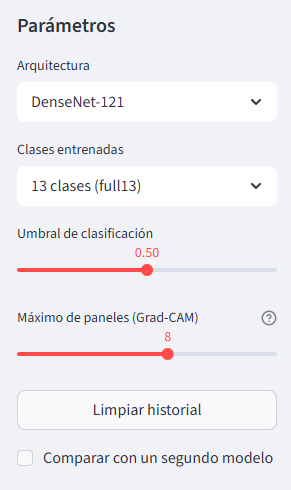
\includegraphics[width=0.30\textwidth]{figures/web/zona-parametros_1_modelo.png}\\[10pt]
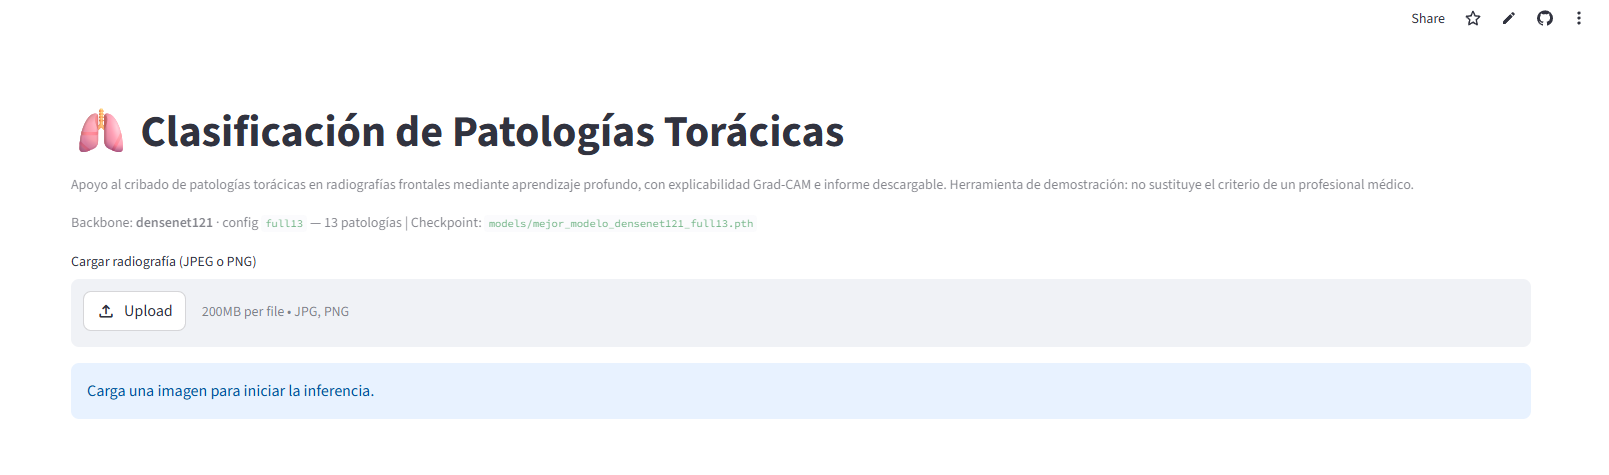
\includegraphics[width=\textwidth]{figures/web/zona-carga.png}
\caption{Configuración del modelo y de los parámetros en la barra lateral (arriba) y
carga de la radiografía (abajo).}
\label{fig::anexo_web1}
\end{figure}

\begin{figure}[ht]
\centering
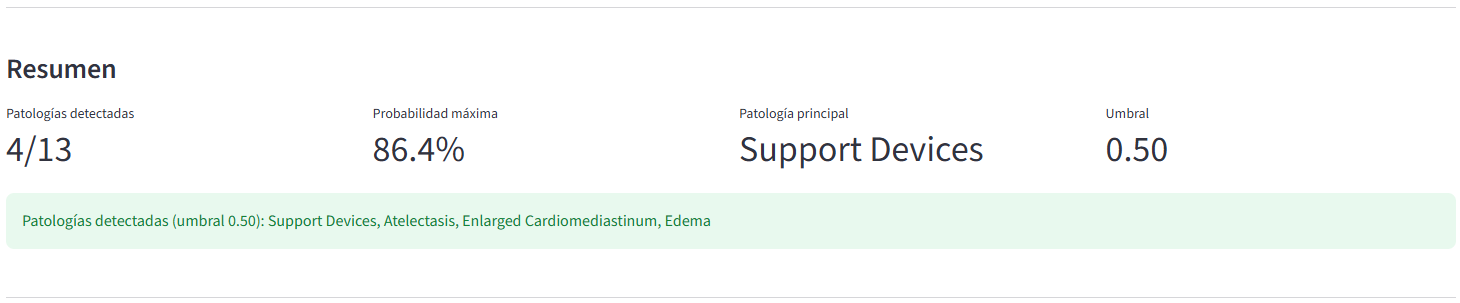
\includegraphics[width=\textwidth]{figures/web/zona_resumen.png}\\[10pt]
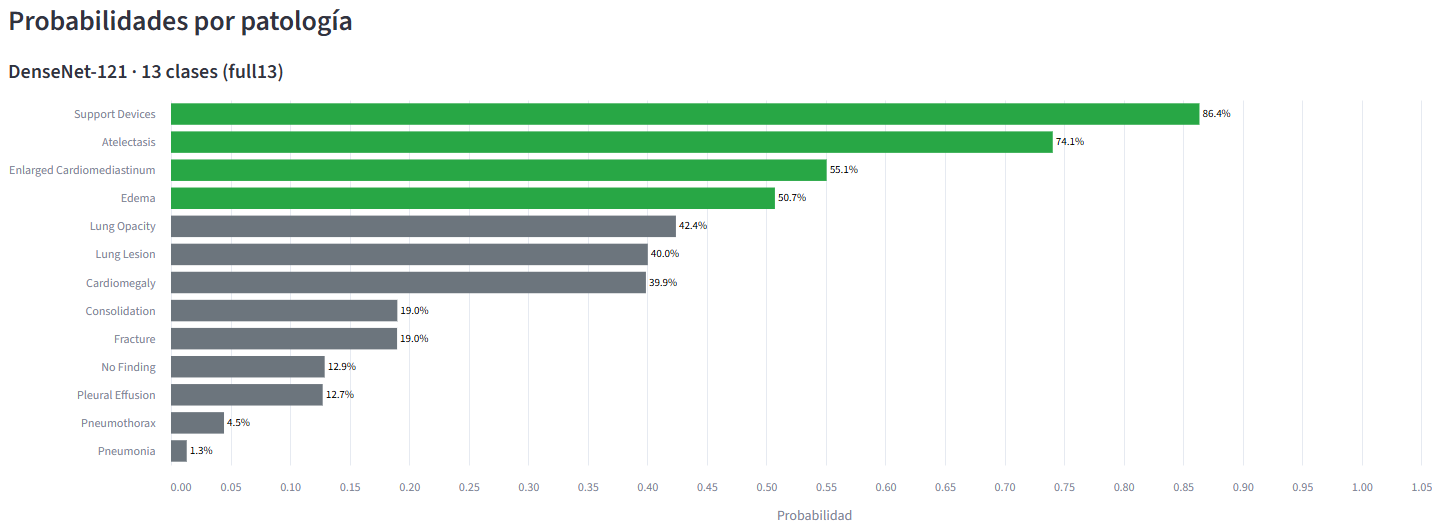
\includegraphics[width=\textwidth]{figures/web/zona-probabilidad-modelo-A.png}
\caption{Resumen de resultados con las tarjetas principales (arriba) y panel de
probabilidades por patología (abajo).}
\label{fig::anexo_web2}
\end{figure}

\begin{figure}[ht]
\centering
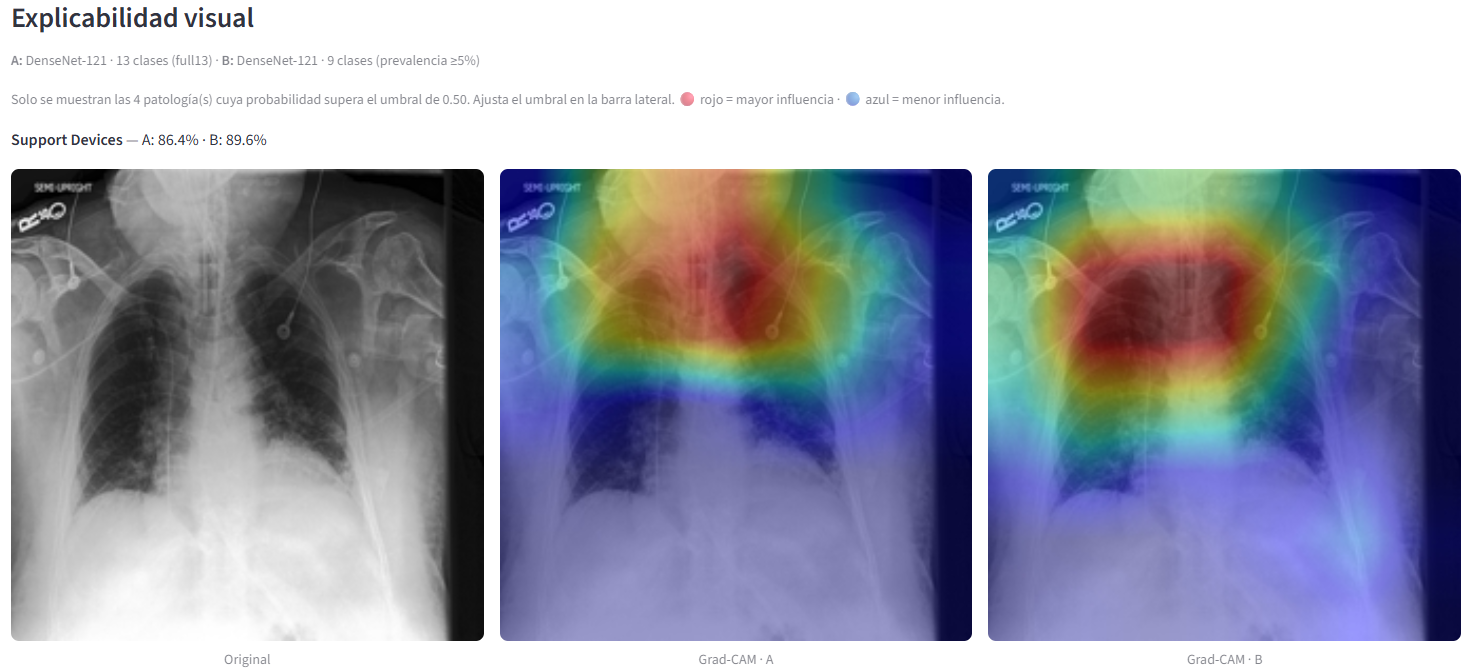
\includegraphics[width=0.85\textwidth]{figures/web/zona-explicabilidad-visual.png}
\caption{Explicabilidad visual: para cada patología detectada, la radiografía original y
su mapa de calor Grad-CAM superpuesto.}
\label{fig::anexo_web3}
\end{figure}

\begin{figure}[ht]
\centering

\includegraphics[width=\textwidth]{figures/web/zona-exportar.png}\\[10pt]
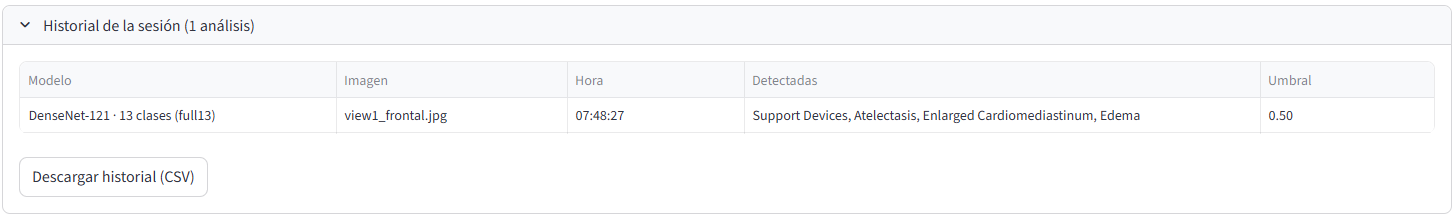
\includegraphics[width=\textwidth]{figures/web/zona-historial-sesion.png}
\caption{Opciones de descarga del informe y de las imágenes (arriba) e historial de la
sesión (abajo).}
\label{fig::anexo_web4}
\end{figure}

\section{Comparación de dos modelos}
\label{anexo::web_comparacion}

La aplicación incorpora un modo de comparación: al activarlo y seleccionar un segundo
modelo, las probabilidades se presentan para cada modelo y sobre las patologías comunes
(Figura~\ref{fig::anexo_comp1}), junto con la tabla de la diferencia absoluta entre ambos
(Figura~\ref{fig::anexo_comp2}); la explicabilidad muestra, además, el mapa Grad-CAM de
los dos modelos por patología (Figura~\ref{fig::anexo_gradcam}).

\begin{figure}[ht]
\centering
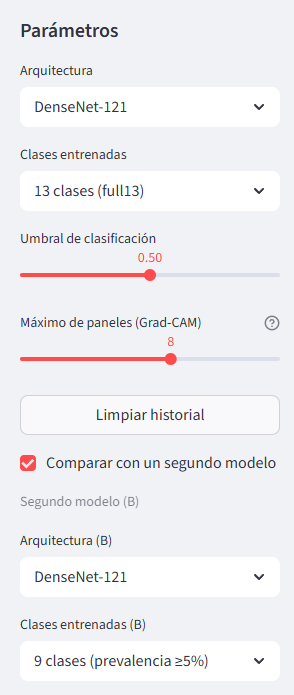
\includegraphics[width=0.27\textwidth]{figures/web/zona-parametros_2_modelos.png}\\[10pt]
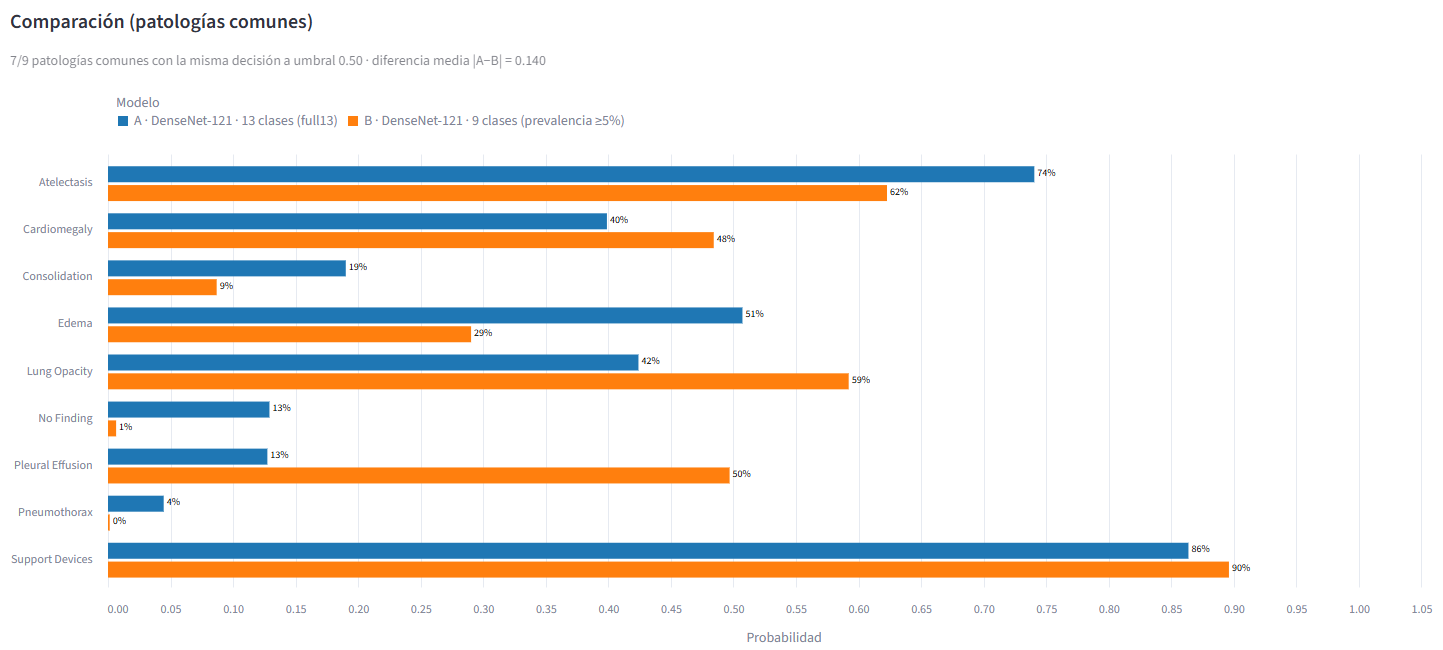
\includegraphics[width=\textwidth]{figures/web/zona-comparacion-patologias-comunes.png}
\caption{Modo de comparación de dos modelos: selección de ambos modelos (arriba) y
gráfica comparativa sobre las patologías comunes (abajo).}
\label{fig::anexo_comp1}
\end{figure}

\begin{figure}[ht]
\centering
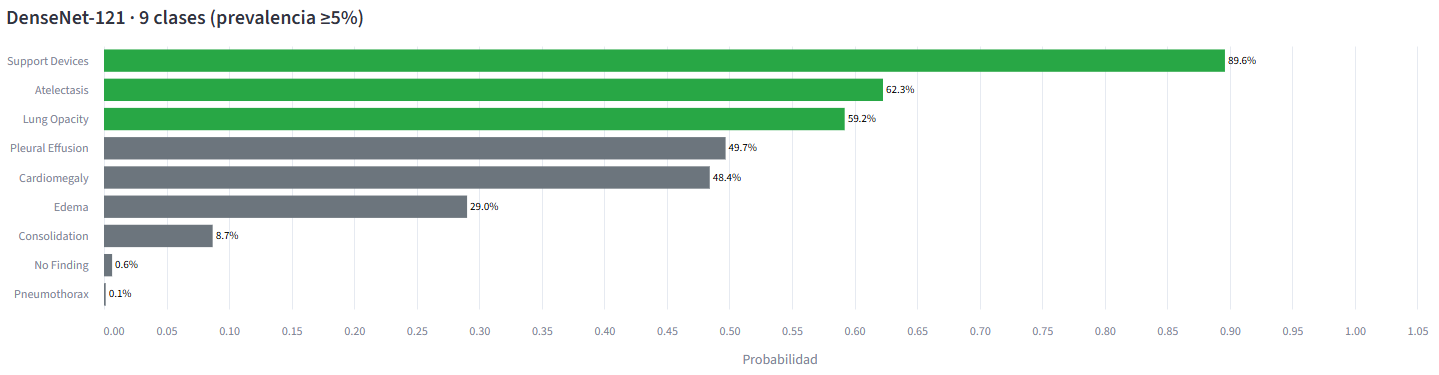
\includegraphics[width=\textwidth]{figures/web/zona-probabilidad-modelo-B.png}\\[10pt]
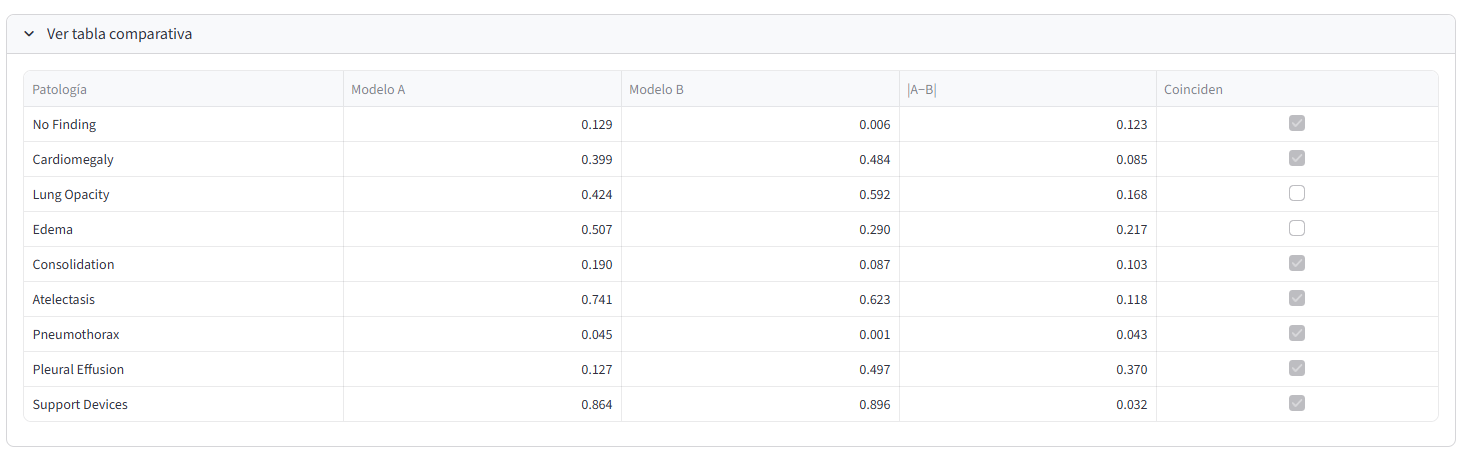
\includegraphics[width=\textwidth]{figures/web/zona-tabla-comparativa.png}
\caption{Comparación de dos modelos: probabilidades del segundo modelo (arriba) y tabla
con la diferencia absoluta entre ambos por patología (abajo).}
\label{fig::anexo_comp2}
\end{figure}

\begin{figure}[ht]
\centering
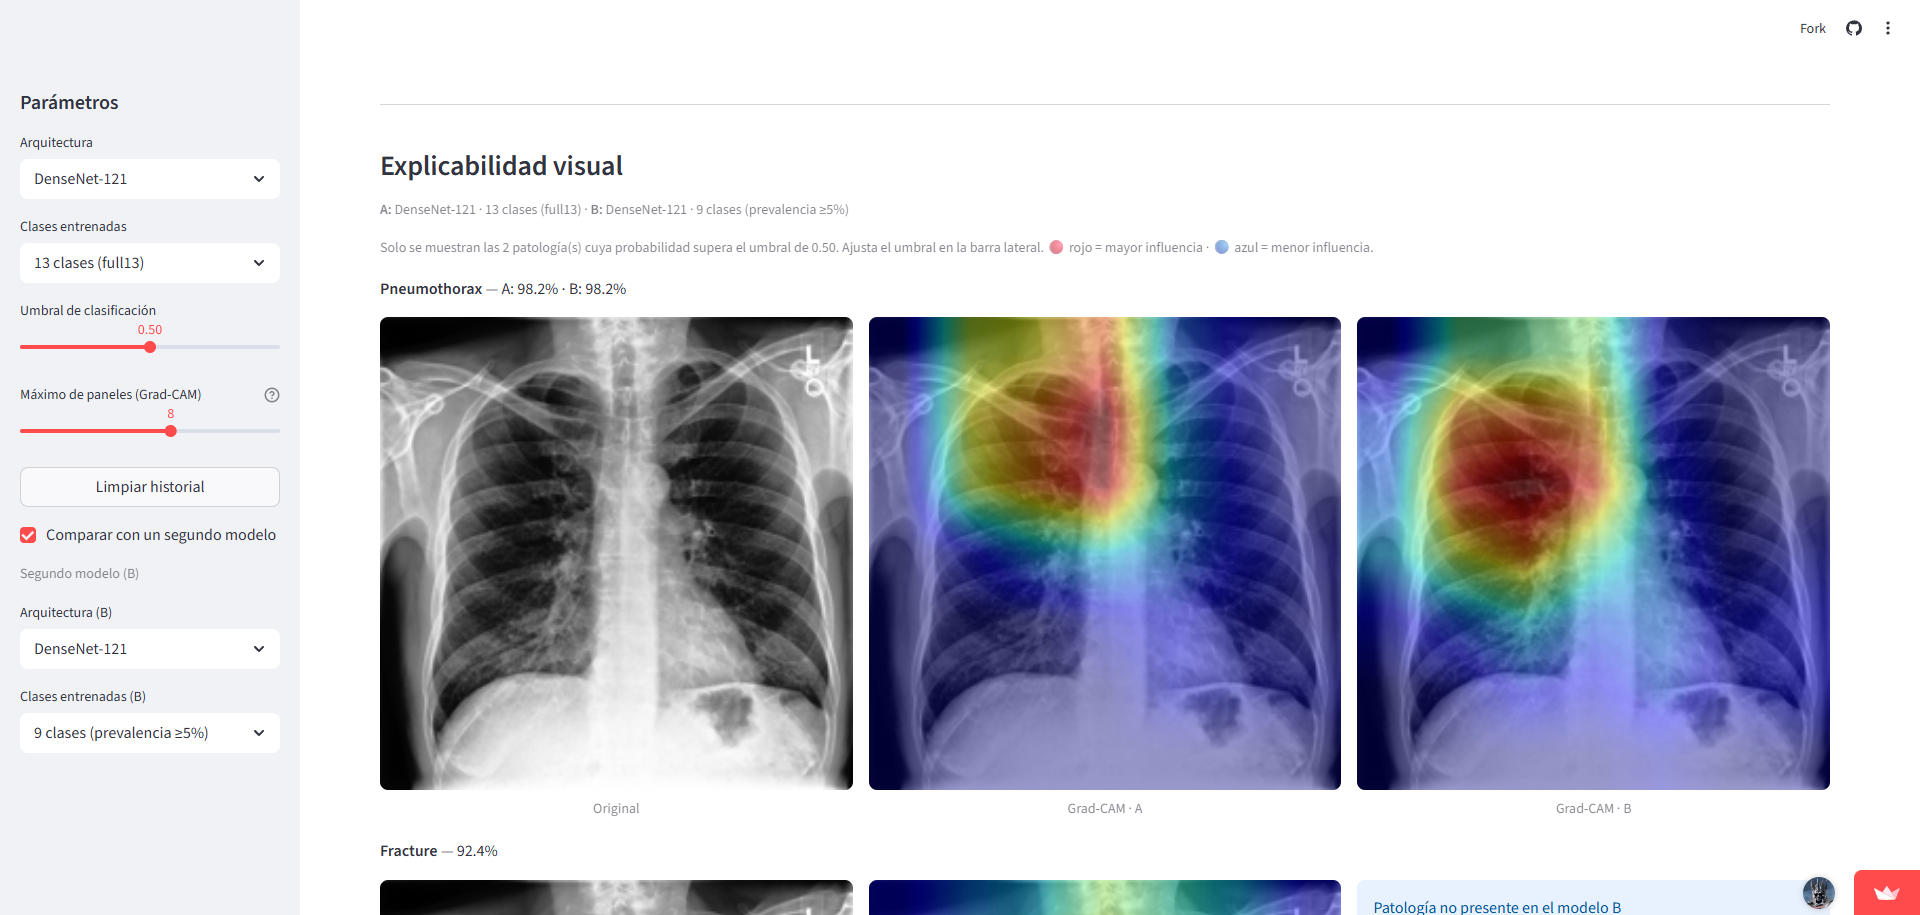
\includegraphics[width=\textwidth]{figures/annexes/gradcam-app_2_modelos.png}
\caption{Explicabilidad comparada: mapas de calor Grad-CAM de los dos modelos sobre una
misma radiografía.}
\label{fig::anexo_gradcam}
\end{figure}

\section{Informe completo generado}
\label{anexo::web_informe}

La aplicación genera un informe PDF descargable que recoge, de forma estructurada, todos
los resultados de la sesión. Las Figuras~\ref{fig::anexo_informe1}
a~\ref{fig::anexo_informe4} reproducen un ejemplo completo (ocho páginas) correspondiente
a una comparación de dos modelos: metadatos de la predicción, tablas y gráficas de
probabilidades de cada modelo, comparación sobre las patologías comunes, explicabilidad
Grad-CAM por patología y un bloque final de métricas de fiabilidad validadas, cerrado con
una advertencia explícita sobre su carácter de herramienta de apoyo y no de diagnóstico.

\newcommand{\pdfinforme}[1]{\includegraphics[page=#1,width=0.47\textwidth]{figures/annexes/Informe_radiologico_torax_20260613_011921.pdf}}

\begin{figure}[ht]
\centering
\pdfinforme{1}\hfill\pdfinforme{2}
\caption{Informe PDF generado por la aplicación (páginas 1 y 2 de 8).}
\label{fig::anexo_informe1}
\end{figure}

\begin{figure}[ht]
\centering
\pdfinforme{3}\hfill\pdfinforme{4}
\caption{Informe PDF generado por la aplicación (páginas 3 y 4 de 8).}
\label{fig::anexo_informe2}
\end{figure}

\begin{figure}[ht]
\centering
\pdfinforme{5}\hfill\pdfinforme{6}
\caption{Informe PDF generado por la aplicación (páginas 5 y 6 de 8).}
\label{fig::anexo_informe3}
\end{figure}

\begin{figure}[ht]
\centering
\pdfinforme{7}\hfill\pdfinforme{8}
\caption{Informe PDF generado por la aplicación (páginas 7 y 8 de 8).}
\label{fig::anexo_informe4}
\end{figure}
